This chapter presents methods used to evaluate the system and the results collected evaluating the system. 

\section{Methods}

\subsection{User Survey}

The system is measured by doing user surveys on the end users. User servery's are done by letting academy coaches answer a couple questions rated on Likert-scale. The questions compares the system against other systems in use at Alfheim today. The Likert-scale chosen is a 5 point scale from \textit{strongly disagree} to \textit{strongly agree}.\footnote{http://www.simplypsychology.org/likert-scale.html}. In short it will let each individual to note how much they disagree or agree with a particular statement.

\subsection{Experiments and Results}

\subsection{Test data}

In the tests Tromsø IL academy coaches has been evaluating the system. In the evaluation phase the database had been populated with data from Tromsø IL and Strømsgodset Toppfotball matches. Only attacks from these two teams has been used in the evaluating process. A total of 34 attacks has been captured for Strømsgodset over 5 matches. For Tromsø a total of 42 attacks has been captured over 9 matches. Figure \ref{fig:matches_regged} lists all matches. Some matches includes data from other teams than Tromsø and Strømsgodset. They have not been taken into consideration in the evaluating process.

\begin{figure}[ht!]
\centering
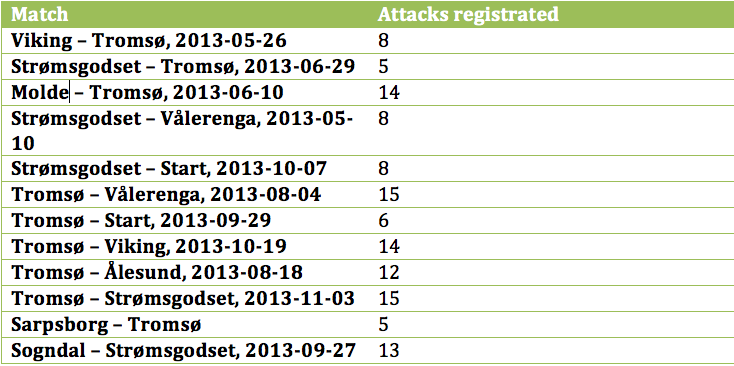
\includegraphics[width=1\textwidth]{images/general/matched_regged.png}
\caption{Matches that have been captured and persisted into the database}
\label{fig:matches_regged}
\end{figure}


\section{Limitations}

As the input is manual the current biggest limitations is humans. 

The input is to some degree subjective for some data like identifying breakthroughs.